\documentclass[aspectratio=169]{beamer}
\usepackage{appendixnumberbeamer}
\usetheme{metropolis}           % Use metropolis theme
\definecolor{fhggreen}{RGB}{23,156,125}
\let\oldemph\textbf
\renewcommand{\textbf}[1]{{\color{mLightBrown}\oldemph{#1}}}

\usepackage{blkarray}
\usepackage{amsmath}
\usepackage{multirow}
\title{The GNU Name System\\\small{secdispatch -- IETF 108}\\\small{\url{https://datatracker.ietf.org/doc/draft-schanzen-gns/}}}
\date{30/7/2020}
\author{Martin Schanzenbach\\Christian Grothoff\\Bernd Fix}
\institute{\hfill\large{GNUnet} 
\includegraphics[trim={0cm 1.5cm 0cm 0cm},clip,width=4em]{gnunet}}
\begin{document}
  \metroset{block=fill,sectionpage=progressbar,numbering=counter}
  \maketitle

\section{The GNU Name System In a Nutshell}
\begin{frame}{Motivation}
  \begin{itemize}
    \item DNS remains a source of traffic amplification DDoS.
    \item DNS censorship (i.e. by China) causes collateral damage in other countries.
    \item DNS is part of the mass surveillance apparatus (MCB).
    \item DNS is abused for offensive cyber war (QUANTUMDNS).
    \item DoT/DoH, DNSSEC, DPRIVE unfortunately do \textbf{NOT} fix this.
  \end{itemize}
\end{frame}

\begin{frame}{What is the GNU Name System?\footnote{Joint work with Christian Grothoff and Matthias Wachs}}
  \begin{itemize}
    \item Fully decentralized name system $\Rightarrow$ Names are not global.
    \item Supports globally unique and secure identification.
    \item Features query and response privacy.
    \item Provides a public key infrastructure
      \begin{itemize}
        \item Each zone is associated with a cryptographic key pair.
        \item Delegation between zones establishes trust relationship.
      \end{itemize}
    \item Interoperable with DNS.
    \item Usable.\footnote{User studies conducted in ``Decentralized Authentication for Self-Sovereign Identities using Name Systems'' (DASEIN) project.}
  \end{itemize}
\end{frame}

\begin{frame}{Applications}
  \begin{itemize}
    \item Identity management: \textbf{re:claimID} (\url{https://reclaim-identity.io})
    \item Social Networks: \textbf{SecuShare} (\url{https://secushare.org})
    \item Healthcare and IoT: \textbf{Accident insurance and private health data}.\footnote{Joint work with University of Applied Sciences Bern, ``Decentralized Authentication for Self-Sovereign Identities using Name Systems'' (DASEIN)}
    \item Others: \textbf{Chat}, \textbf{Host addressing}, \ldots
  \end{itemize}
\end{frame}

\section{Technical Overview}
\begin{frame}{Record Storage / Retrieval}
  \begin{itemize}
    \item GNS stores records in a \textbf{Distributed Hash Table} (DHT).
    \item DHTs allow us to map keys to values.
    \item Naive approach: Map domain names to records.\\e.g.: example.com $\Rightarrow$ A: 1.2.3.4
  \end{itemize}
  \begin{center}
    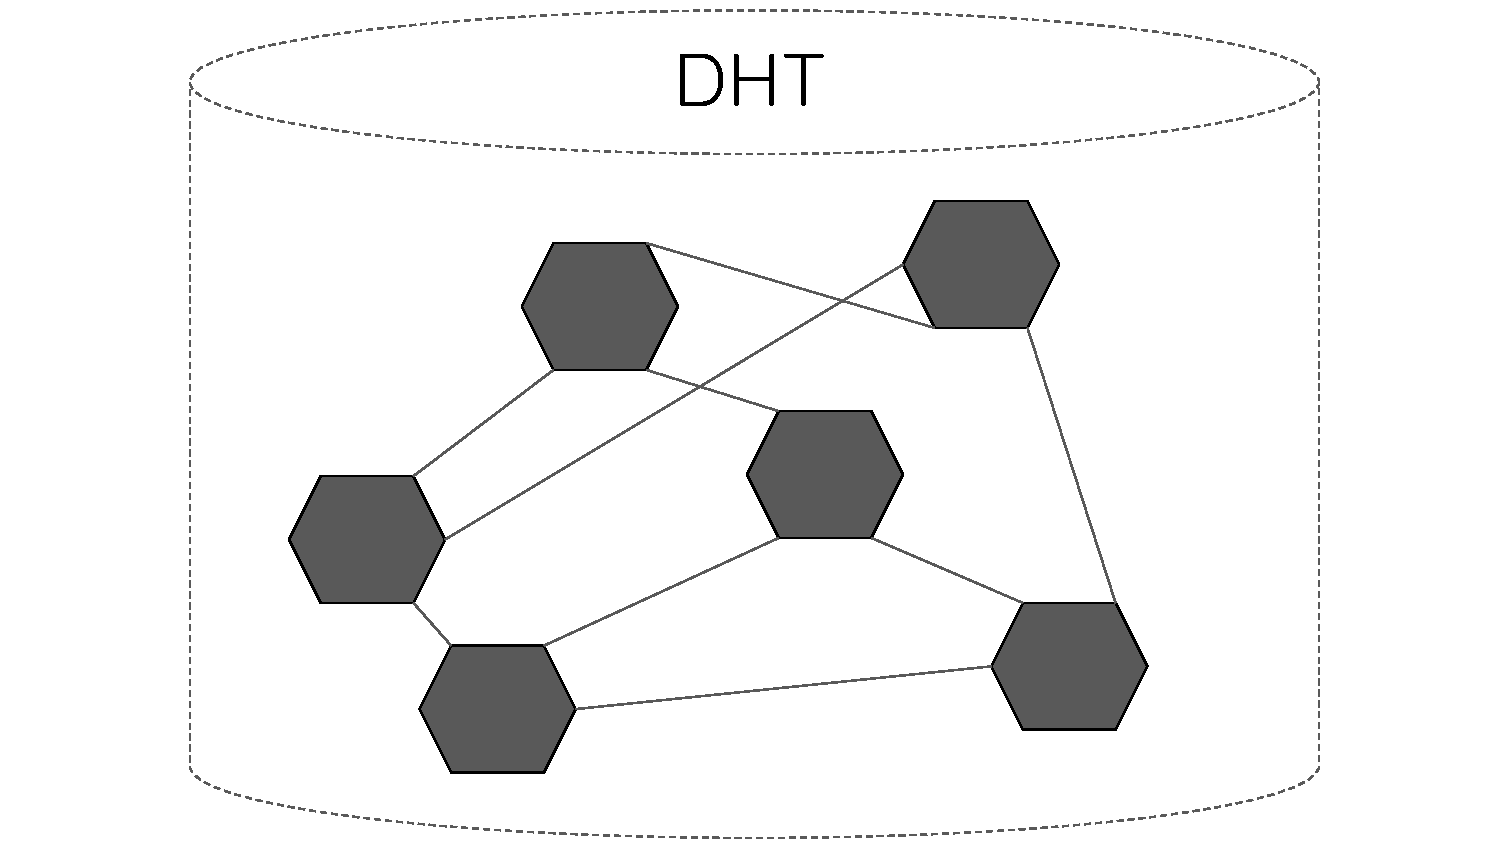
\includegraphics[width=0.5\textwidth]{DHT.pdf}
  \end{center}
\end{frame}

%\begin{frame}{Record Storage / Retrieval}
%  \begin{itemize}
%    \item GNS implements a \textbf{Private Information Retrieval} (PIR) scheme.
%    \item DHT values (records) are signed and encrypted.
%    \item DHT keys are derived from queried name and zone.
%  \end{itemize}
%  \begin{center}
%    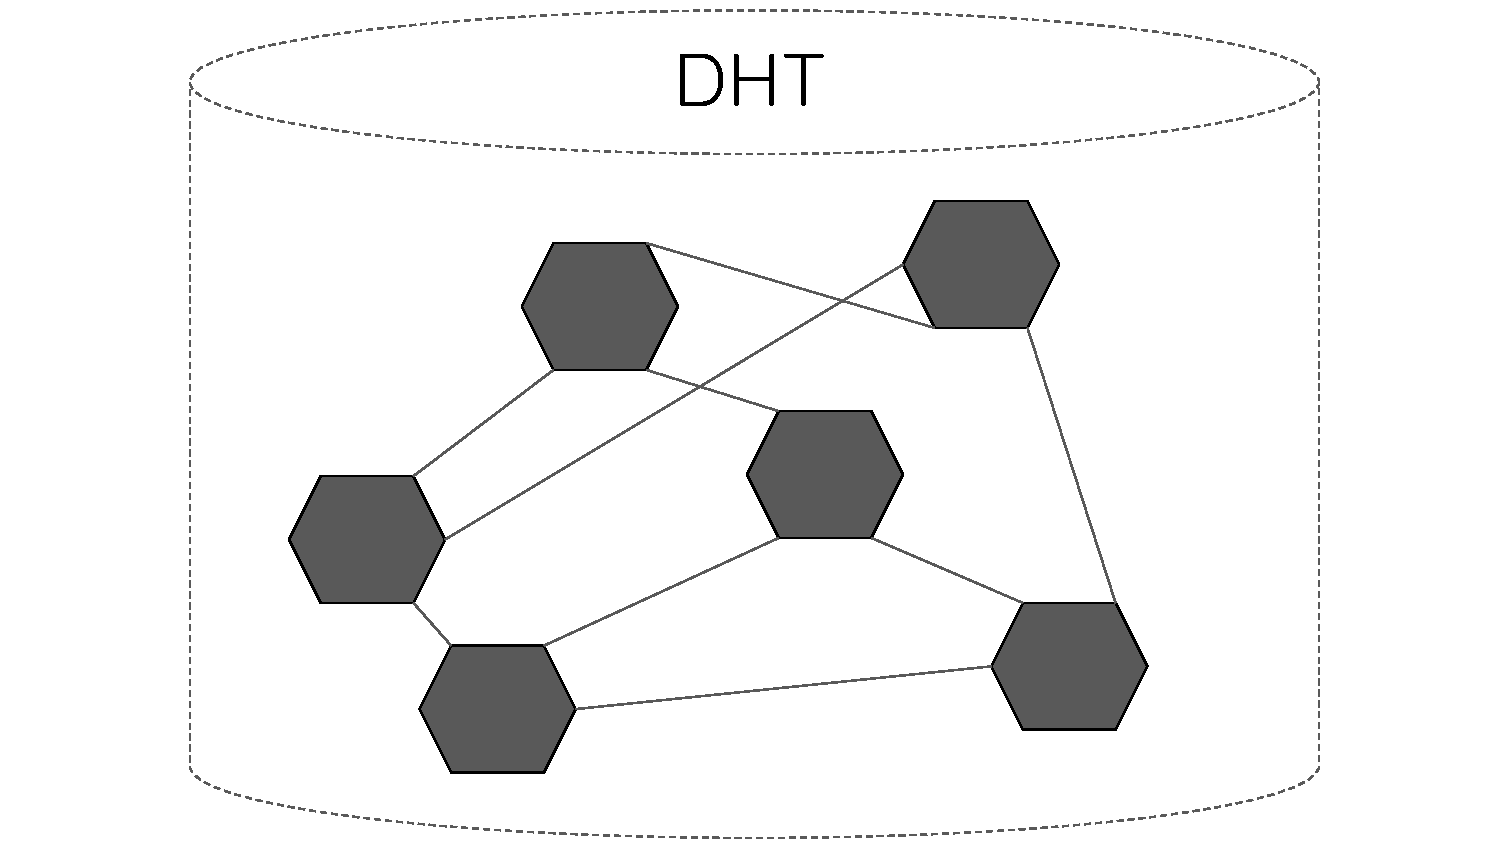
\includegraphics[width=0.5\textwidth]{DHT.pdf}
%  \end{center}
%\end{frame}

\begin{frame}{Secure Storage / Retrieval}
   \begin{itemize}
    \item \textbf{Query privacy}
      \begin{itemize}
        \item GNS implements a \textbf{Private Information Retrieval} (PIR) scheme:\\
  ``a protocol that allows a user to retrieve an item from a server in possession of a database without revealing which item is retrieved.''\footnote{\url{https://en.wikipedia.org/wiki/Private_information_retrieval}}

        \item Queries do not reveal domain name.
        %item DHT keys are ``blinded'' record labels and zone identity.
      \end{itemize}
    \item \textbf{Record confidentiality}: Values in DHT are signed and encrypted by zone owner.
    \item \textbf{Zone privacy}: Zones cannot be enumerated.
    \item \textbf{Censorship and DDoS resistance}: Decentralized, resilient directory.
  \end{itemize}
\end{frame}

\begin{frame}{Zone Delegation}
  \begin{itemize}
    \item The ``NS'' equivalent in GNS is called ``PKEY''.
    \item A ``PKEY'' record contains public zone keys.
    \item The combination of a ``PKEY'' record value and a name allows users to
      query records in a delegated zone.
  \end{itemize}
\end{frame}

\begin{frame}
  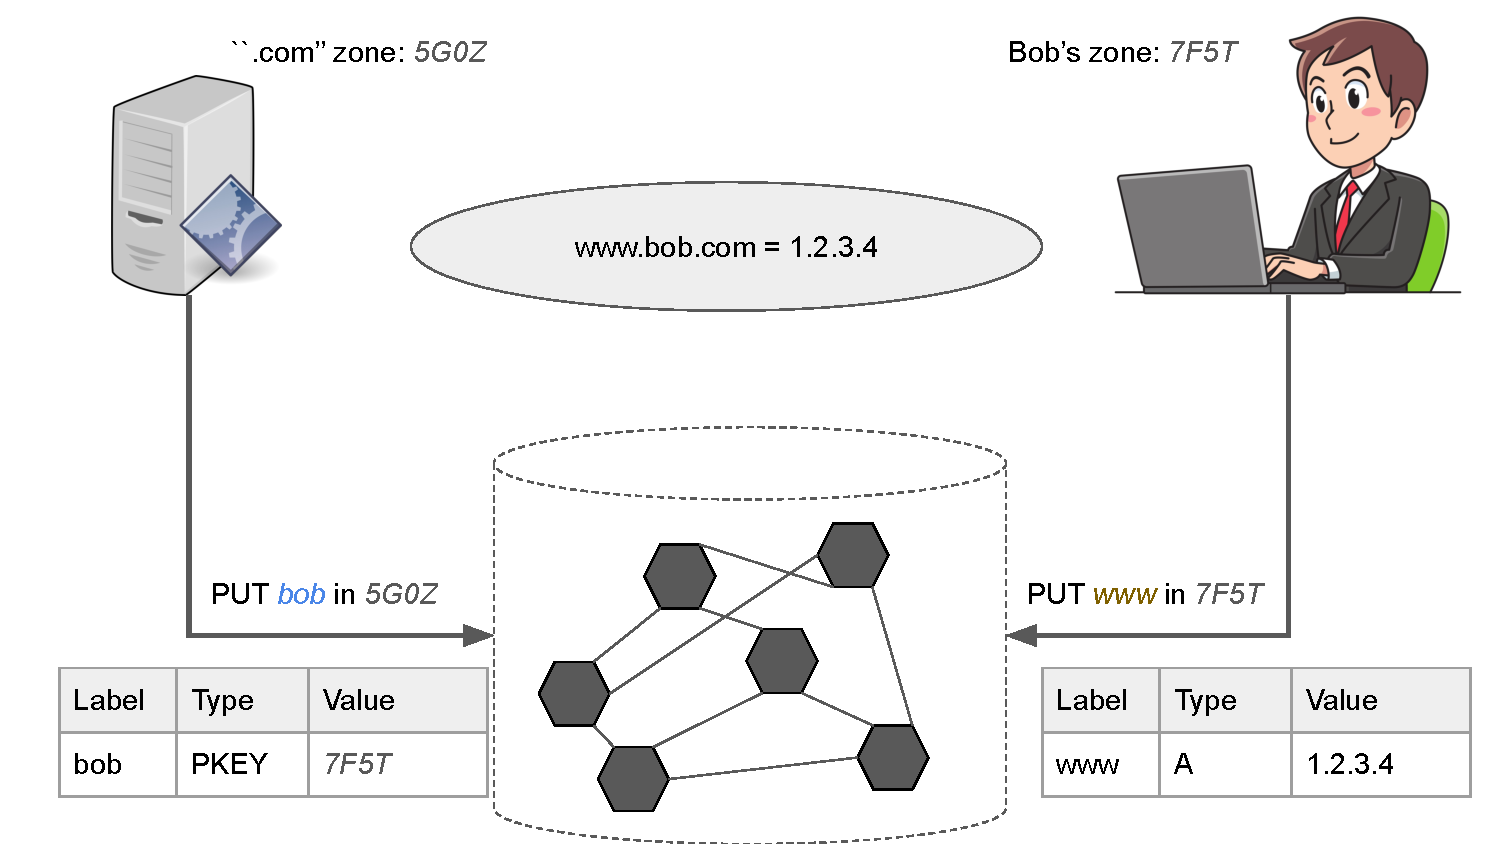
\includegraphics[height=0.9\textheight]{deleg0.pdf}
\end{frame}


\begin{frame}
  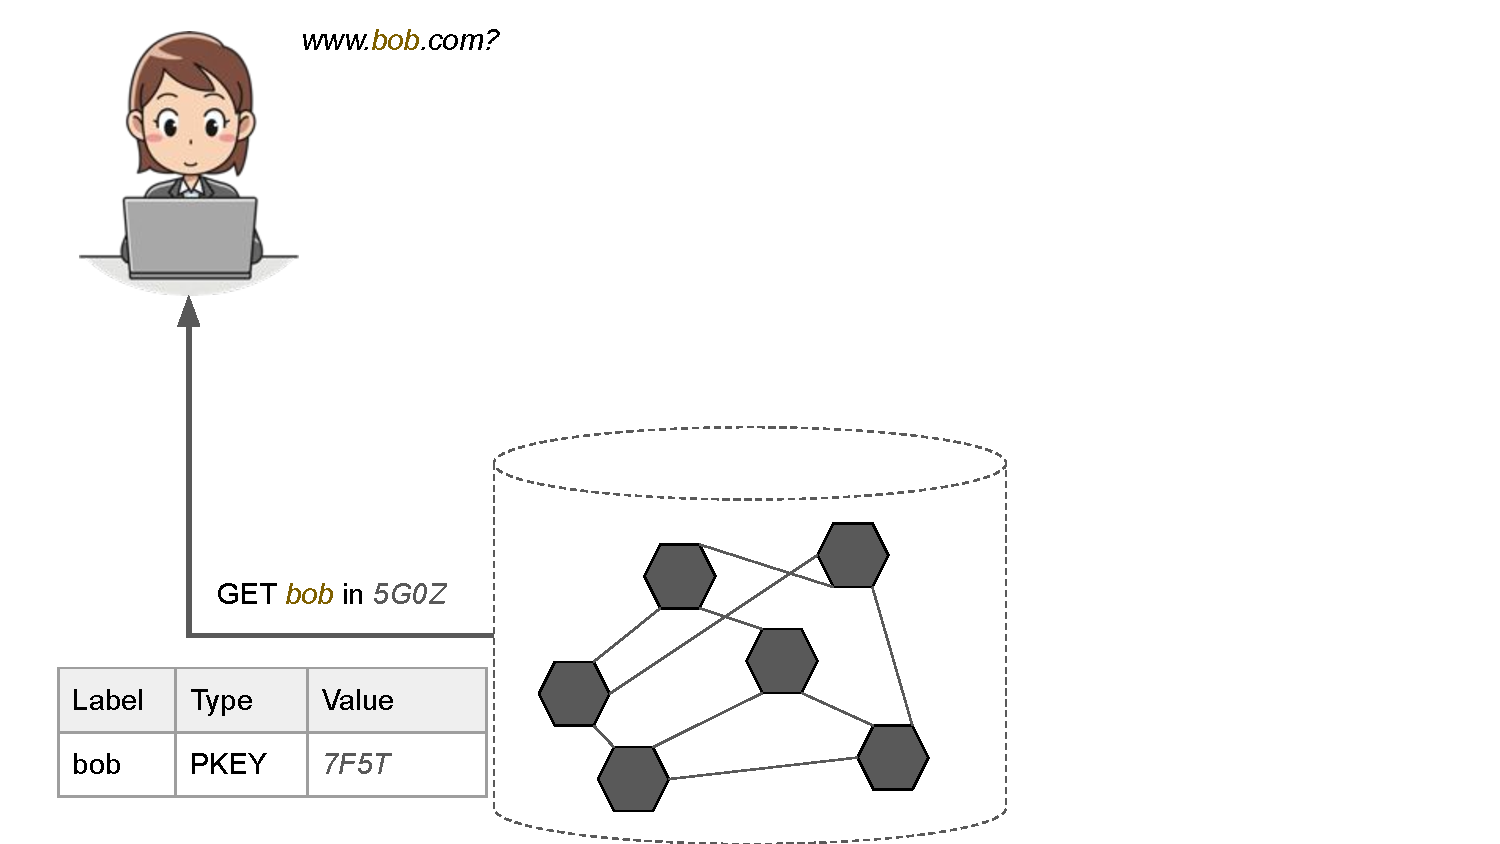
\includegraphics[height=0.9\textheight]{deleg1.pdf}
\end{frame}


\begin{frame}
  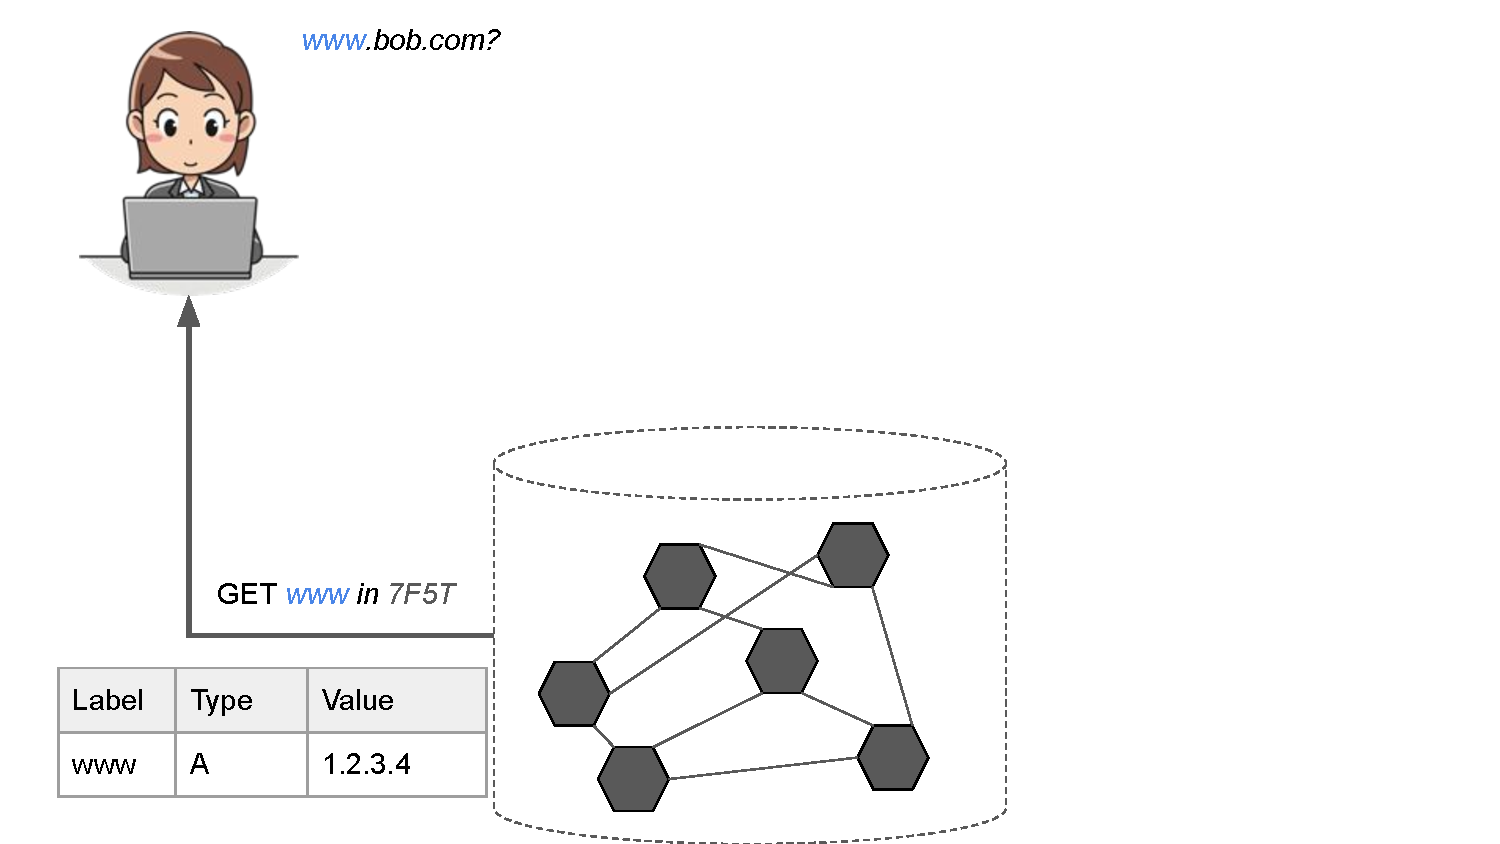
\includegraphics[height=0.9\textheight]{deleg2.pdf}
\end{frame}

\section{Why are we here?}
\begin{frame}{Discussions at IETF/W3C/ICANN}
  \begin{itemize}
    \item IETF 93: \url{https://datatracker.ietf.org/doc/slides-93-dnsop-5/}
      \begin{itemize}
        \item Failed attempt to special-use '.gnu' for GNS.
        \item Resulting in RFC7686, RFC8244
      \end{itemize}
    \item STRINT 2014 (W3C/IAB workshop): \url{https://grothoff.org/christian/strint2014.pdf}
    \item IETF 104 IRTF DINRG WG: \url{https://datatracker.ietf.org/doc/slides-104-dinrg-gnu-name-system/}
    \item ICANN66: \url{https://git.gnunet.org/presentations.git/plain/icann66/20191105_icann66_gns.pdf}
  \end{itemize}
\end{frame}


\begin{frame}{Current Status}
  \begin{itemize}
    \item Who is (and will be) working on it:
      \begin{itemize}
        \item GNUnet project.
        \item Current funding for specfication by NLnet: \url{https://nlnet.nl/project/GNS/}.
      \end{itemize}
    \item Implementation
      \begin{itemize}
        \item Reference implementation in C part of GNUnet: \url{https://git.gnunet.org/gnunet.git/tree/src/gns}
        \item Second implementation in Go: https://github.com/bfix/gnunet-go/tree/master/src/gnunet/service/gns
      \end{itemize}
    \item Specification
      \begin{itemize}
        \item Current draft: \texttt{draft-schanzen-gns-01}.
        \item Status: Documents current implementation. Collecting feedback to improve protocol (and spec).
      \end{itemize}
  \end{itemize}
\end{frame}

\begin{frame}{Next steps}
  \begin{itemize}
    \item Address received feedback:
      \begin{itemize}
        \item Better trust agility to address questions on choice of Hierarchical Deterministic Key Derivation (HKDF). No "standard" go-to HKDF exists at this time:
          \begin{itemize}
            \item In draft and implemented: ECDSA (RFC6979) over Curve25519 (RFC8031).
            \item Alternatives: Schnorr/Ed25519-based (``Tor-style'').\footnote{BIP32-Ed25519 has issues: \url{https://forum.web3.foundation/t/key-recovery-attack-on-bip32-ed25519/44}}
          \end{itemize}
        \item Update to symmetric encryption scheme for IND-CCA.
        \item Address other feedback.
      \end{itemize}
    \item Desired next steps at IETF:
  \begin{itemize}
    \item Receive feedback from IETF experts on protocol and document.
    \item Is this document interesting to any existing IETF/IRTF WG? Should/can a new WG be formed?
  \end{itemize}
  \end{itemize}
\end{frame}



\begin{frame}
  \begin{center}
    The GNU Name System\\
    \vspace{2cm}
    \url{https://gnunet.org}\\
    \vspace{1em}
    {\tiny
    \texttt{schanzen@gnunet.org}\\
    \texttt{3D11~063C~10F9~8D14~BD24~D147~0B09~98EF~86F5~9B6A}\\
    }
  \end{center}
\end{frame}

\appendix

\begin{frame}{References}
  \centering
  {\small
  \begin{enumerate}
    \item {Matthias Wachs, Martin Schanzenbach and Christian Grothoff. {\em A Censorship-Resistant, Privacy-Enhancing and Fully Decentralized Name System}. {\bf 13th Intern
      ational Conference on Cryptology and Network Security}, 2014.}
    \item {Martin Schanzenbach, Georg Bramm, Julian Schütte. {\em reclaimID: Secure, Self-Sovereign Identities Using Name Systems and Attribute-Based Encryption}. {\bf 17th
      IEEE International Conference On Trust, Security And Privacy In Computing And Communications (TrustCom)}, 2018}
    \item {Christian Grothoff, Martin Schanzenbach, Annett Laube, Emmanuel Benoist, Pascal Mainini. {\em Decentralized Authentication for Self-Sovereign Identities using Name Systems (DASEIN)}. {\bf https://git.gnunet.org/bibliography.git/plain/docs/dasein10.pdf}, 2018.}
  \end{enumerate}
  }
\end{frame}

\section{How do we bootstrap the top-level zones?}
\begin{frame}
  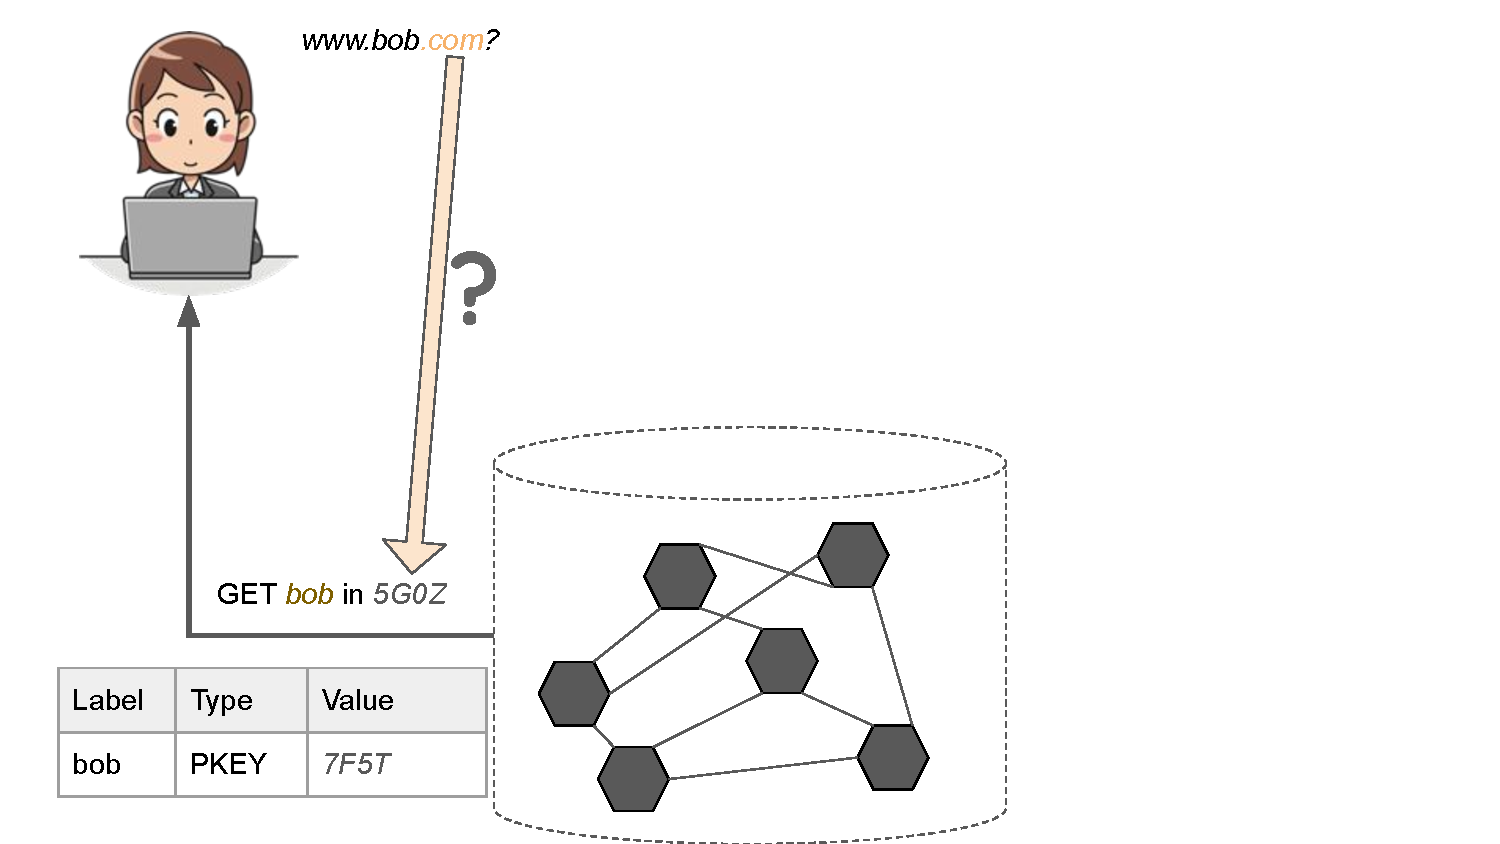
\includegraphics[height=0.9\textheight]{deleg3.pdf}
\end{frame}


\begin{frame}{The GNU Name System Root}
  ``Hyper-hyper local root'' concept:
  \begin{itemize}
    \item Resolver ships with initial root zone configuration.
    \item Root zone configurable \emph{locally} at \emph{each} endpoint.
    \item User override/extension of root at top-level or subdomain-level for:
      \begin{itemize}
        \item Circumvent censorship if necessary.
        \item Private networks.
      \end{itemize}
  \end{itemize}
\end{frame}

\begin{frame}{Envisioned Governance Model}
  \begin{itemize}
    \item Non-profit organization.
    \item Multi-stakeholder model: Board, supporting organizations, \ldots
    \item Examples for possible stakeholders:
      \begin{itemize}
        \item Software and OS Distributors
        \item Browser vendors
        \item Governments
      \end{itemize}
    \item Funding options:
      \begin{itemize}
        \item Applications for new top-level domains.
        \item Registrations of new top-level domains.
        \item \ldots
      \end{itemize}
  \end{itemize}
\end{frame}


\end{document}
